\documentclass[conference]{IEEEtran}
% \IEEEoverridecommandlockouts
% The preceding line is only needed to identify funding in the first footnote. If that is unneeded, please comment it out.
\usepackage{cite}
\usepackage{amsmath,amssymb,amsfonts}
\usepackage{algorithmic}
\usepackage{algorithm}
\usepackage{graphicx}
\usepackage{textcomp}
\usepackage{hyperref}
\usepackage{subcaption}
\usepackage{xcolor}
\newcommand{\todo}[1]{\textcolor{red}{#1}}

\def\BibTeX{{\rm B\kern-.05em{\sc i\kern-.025em b}\kern-.08em
    T\kern-.1667em\lower.7ex\hbox{E}\kern-.125emX}}
\begin{document}

%\title{Audio restoration using plug-and-play approach\\
%	{}
%\thanks{Identify applicable funding agency here. If none, delete this.}
%}

\title{Joint audio denoising and inpainting with plug-and-play proximal algorithm}

\author{\IEEEauthorblockN{Michal Švento}
%\IEEEauthorblockA{\textit{dept. name of organization (of Aff.)} \\
%\textit{Brno University of Technology}\\
%Brno, Czech Republic \\
%212584@vut.cz}
\IEEEauthorblockA{
	\textit{Brno University of Technology, FEEC,} \\
	\textit{Department of Telecommunications,} \\
	Technická 12, 616 00 Brno, Czech Republic \\
	\href{mailto:212584@vut.cz}{212584@vut.cz}
}
\and
\IEEEauthorblockN{Ondřej Mokrý}
%\IEEEauthorblockA{\textit{Signal Processing Laboratory} \\
%\textit{Brno University of Technology}\\
%Brno, Czech Republic \\
%xmokry12@vut.cz}
\IEEEauthorblockA{
	\textit{Brno University of Technology, FEEC,} \\
	\textit{Department of Telecommunications,} \\
	Technická 12, 616 00 Brno, Czech Republic \\
	\href{mailto:xmokry12@vut.cz}{xmokry12@vut.cz}
}
}

\maketitle

\begin{abstract}
We propose plug-and-play variant of proximal algorithm Douglas--Rachford for audio inpainting.
In our situation, also observed samples are interferenced with noise.
We demonstrate, that plug-and-play has potential to succeed after adding a approximal information about some samples.
In a few metrics increase quality and sensitivity to this parameter is significantly lower than in conventional method. 
%\todo{Navrhujeme plug-and-play variantu proximálního algoritmu Douglas--Rachford pro audio inpainting v situaci, kdy i pozoraované vzorky jsou rušeny šumem.Demonstrujeme, že plug-and-play přístup má potenciál fungovat, přidání nějaké přibližné informace o některých vzorcích v některých metrikách zlepšuje kvalitu a citlivost na tento parametr je výrazně nižší než u konvenční metody.}
\end{abstract}

\begin{IEEEkeywords}
speech enhancement, deep learning, denoising, Douglas--Rachford algorithm, inpainting
\end{IEEEkeywords}

\section{Introduction}

%\todo{\begin{itemize}
%%	\item sjednotit restoration versus reconstruction
%%	\item sjednotit plug-and-play versus Plug-and-Play
%	\item srazit na 4 strany
%	\item popisek obrázku \ref{fig:final2witherrors}
%\end{itemize}}

Audio enhancement tasks mostly face problems like missing or damaged samples, noise, or clipping.
Considering speech signals, we %should not avoid the intelligibility problems.
are not only interested in restoring the degradation sample by sample, but we also aim at improving the intelligibility of the recorded speech.
Each restoration problem has developed its own way of enhancing the signal.
Nowadays, the best way to differentiate algorithms is into two categories:
conventional, e.g.\ using autoregressive (AR) modeling or sparsity-based optimization, and solutions using deep learning.
The present paper focuses on the case of restoring a partially observed signal whose observed samples are further degraded by noise, i.e., the aim is to perform simultaneous inpainting and denoising of the speech signal.

In conventional approaches to inpainting, the AR-based Janssen \cite{Janssen1986} and Etter~\cite{Etter1996} algorithms dominate in terms of restoration quality.
% These approaches are based on autoregressive signal modeling \cite{Mokry2020}.
% Sparse signal representation has changed efficiency of restoration, mainly because increase of computing power.
A more recent, successful class of methods is based on sparsity.
The key idea is that after performing proper time-frequency analysis of an audio signal,
most of the information is concentrated in a few coefficients, i.e., it is sparse.
This can be applied as fitting the sparsest possible restoration either to the reliable observed samples \cite{Adler2012, Kitic2015, Zaviska2019, Mokry2019}, or to a signal not much diverging from the observation in the case of denoising \cite{Kowalski2013}.
% The information hidden in frequency representation (using proper time-frequency analysis) is sparse, i.e. we do not need each spectral coefficient to repair the signal with improved subjective results.
%The most advanced works using sparsity are \cite{Adler2012,Kitic2015,Zaviska2019, Mokry2019}.

Deep learning algorithms have also made their own progress in this area.
The most efficient neural network models are autoencoders,
recurrent neural networks (RNN) and
Generative Adversial Networks (GAN).
Current state-of-the-art deep learned algorithms are Speech Enhancement GAN (SEGAN) \cite{Pascual2017}, NSNet \cite{Xia2020}, FullSubNet \cite{Hao2021}.
While learning-based algorithms allow to adapt to real-world signals, rather than to rely on hand-crafted priors like sparsity or the AR nature of signals, they need large datasets for training.
Furthermore, neural networks are usually trained for a specific problem, lacking universal applicability on similar restoration tasks, in contrast to sparsity-based methods \cite{Gaultier2017, Mokry202021, Zaviska2021}.

As a compromise between the conventional and learning-based methods, 
% In \cite{Chan2016} was introduced plug-and-play method for image restoration.
the plug-and-play method for image restoration was introduced in \cite{Venkatakrishnan2013} and subsequently studied in \cite{Chan2016},
where part of each iteration of an optimization algorithm is replaced by a (learned) denoiser.
% The idea of a hybrid model,
% combining conventional approach (convex minimization) with deep learning,
% has shown succesful.
In the present paper, we propose a hybrid algorithm based on the same paradigm, aiming at restoration of degraded speech.
While \cite{Chan2016} focused on adapting the Alternating Direction method of Multipliers (ADMM) and a recent declipping approach used the learned element only partially \cite{Tanaka2022}, we choose an opposite approach by working with a simple Douglas--Rachford algorithm (DRA) and exploring the trade-off between data fitting and denoising in the algorithm.


%Our motivation is to transform this model to audio problems with minor differences.
%We replace Alternating Direction Multiplier Method (ADMM) with Douglas-Rachford algorithm (DR~algorithm).
%Denoiser will be chosen from state-of-the-art audio denoisers. 

%% Introduction to sections.
The paper is organized as follows. In section \ref{sec:prereq} we introduce the task from mathematical point of view and we define the restoration as a minimization task.
Section \ref{sec:plugaandplay} presents the plug-and-play method and its challenges.
Section \ref{sec:eval} discusses the results and further improvements of algorithm.
Finally, Section \ref{sec:conclusion} concludes the paper.

\section{Prerequsities}\label{sec:prereq} 

%\todo{Asi můžeme nechat obě formulace, protože zapadají do příběhu -- máme formulaci pro koeficienty, která umožňuje formulovat DRA s projekcí a soft. My ale chceme upravovat proximální operátor definovaný na signálu, proto máme druhou formulaci a k ní příslušný (přibližný) algoritmus \ref{alg:DRA_t}.
%U varianty koeficienty bych ale možná nechal formulaci, ale algoritmus \ref{alg:DRA_c} bych možná vypustil.}

In this section, we formalize the task of inpainting and denoising and propose algorithmic solutions based on DRA.
% The proposed method \cite{Chan2016} assumes any damage,
% but we start with missing samples and then expand the model for various damages.
% The rest of the section explains minimization problem solved by DRA.
% Solution has two approaches.
First, using frequency coefficients as input explained in \ref{subsec:freqcoef}~\cite{Mokry2020}.
Second, using samples in time domain is described in subsection \ref{subsec:timecoef} \cite{Mokry2021}.


\subsection{Task formulation}

We consider column vector $ \mathbf{s} \in \mathbb{R}^{N} $ as our observed damaged single-channel signal of length $ N $.
We have set $ I $ of sample indices $ \{1,2,\dots,N\} $, which has two disjunctive subsets: $I_\textup{M} $ for missing positions and $ I_\textup{R} $ stands for reliable positions.
Usually, samples $ \mathbf{s}(I_\textup{R}) $ are considered reliable (undamaged) and $ \mathbf{s}(I_\textup{M}) $ are samples, which we are looking for.
It is common to rewrite it in matrix form:
\begin{equation*}
	\mathbf{s}_{\textup{R}} = \mathbf{M}_{\textup{R}}\mathbf{s},
\end{equation*}
where $\mathbf{M}_\textup{R} \in \mathbb{R} ^ { |I_\textup{R}| \times N}$, with $ |I_\textup{R}|$ denotes the number of indices in the subset $I_\textup{R}$, is the mask matrix, selecting rows from identity matrix corresponding to the indices in $I_\textup{R}$ \cite{Adler2012}.
In words, $\mathbf{M}_{\textup{R}}\mathbf{s}$ represents choosing the samples from $\mathbf{s}$ on positions $I_\textup{R}$.

It is convenient to define the set of signals fitting the observation as
\begin{equation}
	\label{eq:Gamma}
	\Gamma = \lbrace \mathbf{x}\in \mathbb {R}^L\mid \mathbf{M}_{\textup{R}}\mathbf{x}=\mathbf{M}_{\textup{R}}\mathbf {s}\rbrace.
\end{equation}
In the noise-less case, we would search for a suitable signal in $\Gamma$.
On the other hand, when the observed samples are distorted by noise, we only require the solution $\mathbf{x}$ to be close to $\Gamma$.
%\todo{V algoritmech máme proměnnou $\mathbf{x}$ pro signály, tudíž bych ji asi používal už odsud namísto $\mathbf{y}$.}

\subsection{Synthesis-based formulation}\label{subsec:freqcoef}
%\todo{Pro tento přístup se používá označení syntetizující (\textit{synthesis} nebo \textit{synthesis-based formulation}), pro ten v další části analyzující (\textit{analysis}).}

We define the task as of finding a suitable signal in (or close to) $\Gamma$ as a sparsity-based problem, minimizing $ \ell_0 $-norm of the Gabor coefficients, i.e., the number of non-zero coefficients of the time-frequency representation of the signal.
%\todo{(možná hned používat Gabor coefficients, ať dále dává smysl termín Gabor transform)} coefficients of the signal $ \mathbf{s} $.
However, this task leads to an NP-hard problem and is hardly solvable \cite{Mokry2020}.
The closest redefinition is to use the $ \ell_1 $-norm as follows:

\begin{equation}
	\label{eq:synthesis.gamma}
	\mathop {\operatorname{arg \, min}}_\mathbf {c}\Vert \mathbf {c}\Vert _1 \quad \text{subject to}\ \mathbf{D}\mathbf {c}\in \Gamma,
\end{equation} 
where $\mathbf{D} $ is synthesis operator (inverse discrete Gabor transform), which is the adjoint of the analysis operator $ \mathbf{A} $, i.e., $ \mathbf{D} = \mathbf{A}^* $.
Therefore the restored signal corresponds to $ \mathbf {y} =  \mathbf{D}\mathbf {c}$.
% \todo{Je správně $ \mathbf {y} \approx \mathbf{D}\mathbf {c}$, nebo $ \mathbf {y} =  \mathbf{D}\mathbf {c}$? : MŠ: myslím, že rovná sa je správne.}
% \todo{Dal bych asi i $A$ a $\mathbf{D}$ jako matice, i když není nutno.}
% Set $ \Gamma $ is defined as follows:

%\begin{equation}
%	\label{eq:Gamma}
%	\Gamma = \lbrace \mathbf {y}\in \mathbb {R}^L\mid M_{\textup{R}}\mathbf {y}=M_{\textup{R}}\mathbf {s}\rbrace,
%\end{equation}

%One of the suitable solutions is DR algorithm in \ref{alg:DRA_c} \cite{Mokry2020}.
%
%\begin{algorithm}
%	\caption{Douglas-Rachford algorithm -- model with frequency coefficients}
%	\begin{algorithmic}[1]\label{alg:DRA_c}
%		\renewcommand{\algorithmicrequire}{\textbf{Input:}}
%		\renewcommand{\algorithmicensure}{\textbf{Output:}}
%		\REQUIRE  $ \gamma > 0 $, $ \delta  \in (0,1)$ ,
%		
%		\FOR {$n = 0, 1, \dots$}
%		\STATE $\mathbf{\widetilde{c}}_n=\operatorname{proj}_{\Gamma}(\mathbf{c}_n) $ 
%		\STATE $ \mathbf{c}_{n+1} = \mathbf{c}_n + \lambda \left( \operatorname{soft}_{\gamma}\left(2\mathbf{\widetilde{c}}_n-\mathbf{c}_n \right)-\mathbf{\widetilde{c}}_n\right)$
%		\ENDFOR
%		\RETURN $D(\operatorname{proj}_{\Gamma}(\mathbf{c}_n))$ 
%	\end{algorithmic} 
%\end{algorithm}

In the presence of noise, the condition $\mathbf{D}\mathbf {c}\in \Gamma$ is not beneficial, since it forces the solution to still contain the noise.
Its reduction can be included in the formulation by rather minimizing the distance of the solution from the set $\Gamma$.
This can be computed as the difference of the solution $\mathbf{D}\mathbf{c}$ and the observation $\mathbf{s}$  on the positions $I_\textup{R}$.
Typically, squared $\ell_2$-norm is used in this context:
\begin{equation}
	\label{eq:synthesis.dist}
	\mathop {\operatorname{arg \, min}}_\mathbf {c}\Vert \mathbf {c}\Vert _1 + \frac{\alpha}{2} \Vert \mathbf{M}_{\textup{R}} \mathbf{D}\mathbf {c} - \mathbf{M}_{\textup{R}} \mathbf{s} \Vert^2_2.
\end{equation} 
The parameter $\alpha > 0$ manages the trade-off between sparsity of the coefficients and the data-fidelity.

%Operator $ \operatorname{proj}_{\Gamma}(arg)$ is projection onto convex set $ \Gamma $ and $\operatorname{soft}_{\gamma}(arg)$ is soft thresholding operator.
%Both are proximal operators.
%
%The condition   $ \delta  \in (0,1)$ is strict for convergence of solution \cite{Combettes2011}.
Both \eqref{eq:synthesis.gamma} and \eqref{eq:synthesis.dist} could be solved using DRA \cite{Mokry2020, Zaviska2021}.
However, the algorithms use the Gabor coefficients as the main variable, which makes the incorporation of a denoiser (working with a signal as the input) problematic.


\subsection{Analysis-based formulation}\label{subsec:timecoef}

Second approach uses time domain samples as input and also as variables of the optimization task.
In case the transform is redundant, i.e., we have more coefficients than signal samples, this second approach leads to different solutions in general \cite{Mokry2020}. 
% It has mainly computational advice against first approach, signal is typically one dimensional vector, while Gabor coefficients are matrices (e.g less multiplication operations per iteration).
%\todo{OM: tato první věta není úplně pravda, protože v iteraci algoritmu \ref{alg:DRA} pořád máme jednu analýzu a jednu syntézu, stejně jako by tomu bylo v případě syntetizujícím (tam by se ty operátory vyskytovaly uvnitř projekce).}
% \todo{MŠ: Možno nejako takto?}

The main minimazation task \eqref{eq:analysis.gamma} is reformulated as,
\begin{equation}
	\label{eq:analysis.gamma}
	\mathop {\operatorname{arg \, min}}_\mathbf {x}\Vert \mathbf{A} \mathbf {x}\Vert _1 \quad \text{subject to}\ \mathbf {x}\in \Gamma,
\end{equation}
or, in the denoising case,
\begin{equation}
	\label{eq:analysis.dist}
	\mathop {\operatorname{arg \, min}}_\mathbf {x}\Vert \mathbf{A} \mathbf {x}\Vert _1 + \frac{\alpha}{2} \Vert \mathbf{M}_{\textup{R}} \mathbf {x} - \mathbf{M}_{\textup{R}} \mathbf{s} \Vert^2_2.
\end{equation} 
%and $ \Gamma $ is similarly as in \eqref{eq:Gamma} % Tags???????  
%\todo{Tuto rovnici tu máme dvakrát.}
%\begin{equation}
%	\Gamma = \lbrace \mathbf {s}\in \mathbb {R}^N\mid M_{\textup{R}}\mathbf {y}=M_{\textup{R}}\mathbf {s}\rbrace.
%\end{equation}
If we want to employ DRA also on the analysis-based task, a problem occurs
that we do not know proximal operator of $ \ell_1 $-norm after analysis, which is essential for the DRA.
However, we can resort to the so-called approximal operator without significant loss of restoration quality \cite{Mokry2021}.
% OM: Tohle jsme vlastně už řekli v předchozí větě:
%To solve \eqref{eq:analysis.gamma} or \eqref{eq:analysis.dist}, DRA can also be employed, even though it solves only an approximation of the objective \cite{Mokry2021}.
The algorithm is summarized in Alg.\,\ref{alg:DRA}.

% Afterwards our algorithm resolves to following \cite{Mokry2020}: 
\begin{algorithm}
	\caption{DRA for \eqref{eq:analysis.gamma} or \eqref{eq:analysis.dist}.}
	\begin{algorithmic}[1]\label{alg:DRA}
		\renewcommand{\algorithmicrequire}{\textbf{Input:}}
		\renewcommand{\algorithmicensure}{\textbf{Output:}}
		\REQUIRE $ \lambda_n > 0 $, $ \gamma>0 $, $ \mathbf{\widetilde{x}}_0 \in \mathbb{R}^{N} $, $\beta \in [0, 1]$
		\FOR {$n = 0, 1, \dots$}
		\STATE $\mathbf{x}_n= (1-\beta)\mathbf{\widetilde{x}}_n + \beta \operatorname{proj}_{\Gamma}(\mathbf{\widetilde{x}}_n) $ 
		\STATE $ \mathbf{\widetilde{x}}_{n+1} = \mathbf{x}_n + \lambda_n \left( \mathbf{D}\left(\operatorname{soft}_{\gamma}\left(\mathbf{A}\left(2\mathbf{x}_n-\mathbf{\widetilde{x}}_n\right) \right)\right) -\mathbf{x}_n\right)$
		\ENDFOR
		\RETURN $\mathbf{x}_n$ %\todo{DONE:Možná vyměnit značení $\mathbf{\widetilde{x}}$ a $\mathbf{x}$?}
	\end{algorithmic} 
\end{algorithm}

The operator $ \operatorname{proj}_{\Gamma}$ is projection onto convex set $ \Gamma $ and $\operatorname{soft}_{\gamma}$ is soft thresholding operator \cite{Combettes2011}.
Projection, in this case, means replacing restored samples in positions considered reliable by the observed samples.
The parameter $\beta$ allows to differentiate between simple inpainting \eqref{eq:analysis.gamma} and the joint problem \eqref{eq:analysis.dist}.
The case of $\beta = 1$ corresponds to performing projection in the update, in line with \cite{Mokry2020}.
For $\beta < 1$, it can be derived (see e.g.\,\cite[Sec.\,4 and Tab.\,1]{Combettes2011}) that the update corresponds to the proximal operator of $f(\mathbf{x}) = \frac{\alpha}{2} \Vert \mathbf{M}_{\textup{R}} \mathbf {x} - \mathbf{M}_{\textup{R}} \mathbf{s} \Vert^2_2$ with $\alpha = \frac{\beta}{1-\beta}$.


\section{Plug-and-play inpainting} \label{sec:plugaandplay}

The plug-and-play method was proposed in \cite{Venkatakrishnan2013} and \cite{Chan2016} for image restoration.
The main idea is to replace a proximal operator inside an iterative algorithm with an denoiser.
% without any demands from minimizing algorithm (the origin of plug-and-play).
Since this approach does not affect the data-fitting part of the minimization, it should be suitable for different resotaration tasks.
We rewrite this task to solve our audio inpainting problem using DRA with approximal operator (analysis-based), i.e., we modify Alg.\,\ref{alg:DRA}, leading to Alg.\,\ref{alg:pnp}:


\begin{algorithm}
	\caption{Plug-and-play DRA}
	\begin{algorithmic}[1]\label{alg:pnp}
		\renewcommand{\algorithmicrequire}{\textbf{Input:}}
		\renewcommand{\algorithmicensure}{\textbf{Output:}}
		\REQUIRE $ \lambda_n > 0 $, $ \gamma>0 $, $ \mathbf{\widetilde{x}}_0 \in \mathbb{R}^{N} $, $\beta \in [0, 1]$
		\FOR {$n = 0, 1, \dots$}
		\STATE %$\mathbf{\widetilde{x}}_n=\operatorname{proj}_{\Gamma}(\mathbf{x}_n) $ 
		$\mathbf{x}_n= (1-\beta)\mathbf{\widetilde{x}}_n + \beta \operatorname{proj}_{\Gamma}(\mathbf{\widetilde{x}}_n) $ 
		\STATE $ \mathbf{\widetilde{x}}_{n+1} = \mathbf{\widetilde{x}}_n + \lambda_n \left( \mathcal{D} \left(2\mathbf{x}_n-\mathbf{\widetilde{x}}_n \right)-\mathbf{x}_n\right)$
		\ENDFOR
		\RETURN $\mathbf{x}_n$ 
	\end{algorithmic} 
\end{algorithm}

%\subsection{Denoisers}

Convergence of the plug-and-play approach can be proven in case $\mathcal{D}$ is a non-expansive operator \cite{Chan2016}.
However, this is hard to prove in practice with off-the-shelf denoisers.
Thus, the only requirement for our denoiser $\mathcal{D}$ was primarily good results in subjective metrics
(discussed more in \ref{subsec:metrics}).
The implementation of the denoiser of our choice is based on the \textit{mayavoz} toolkit \cite{Shahul2023}.
This tool provides us simple use of learned model with downloadable checkpoints.
Our selection is the WaveUnet learned on the Valentini dateset \cite{ValentiniBotinhao2017} (the variant with 28 speakers).

\section{Testing data and evaluation}\label{sec:eval}

As introduced before, we use discrete Gabor transform as the analysis operator $\mathbf{A}$ with following setup parameters: Gauss window with length $w =1024 $, hop length $a = 256$ and number of frequency channels used in Fast Fourier transform %(FFT)
$n_{\textup{FFT}} = 1024$.
To satisfy the Parseval tight frame condition, the synthesis operator $\mathbf{D} = \mathbf{A}^*$ is configured in the same way \cite{Mokry2020}.

\subsection{Metrics}\label{subsec:metrics}

%\todo{SNR,PESQ,STOI}

A standard metric for restoration quality is the signal-to-noise ratio (SNR), where the \textit{signal} represents the clean ground truth and \textit{noise} is the difference of the restoration and the ground truth.
We calculate SNR either for whole signal or only on $I_\textup{M}$, i.e, on the indices of missing samples.
The higher SNR the better the restoration.

A drawback of SNR is that it measures sample-wise difference, which does not take into account human perception of sound quality.
Valuable metrics for speech signals are those, which measure human perception.
We use two objective metrics: Perceptual Evaluation of Speech Quality (PESQ) \cite{Rix2001} and 
Short-Time Objective Intelligibility (STOI) \cite{Taal2010}.
PESQ has scale from $-0.5$ to $4.5$, with higher score meaning better result.
STOI measures correlation of two signals on a scale from $0$ to $1$.

\subsection{Dataset and degradation setup}
We have chosen to work with
% randomly 10 audio files for final evaluation from 
the Valentini dataset \cite{ValentiniBotinhao2017} used commonly in speech enhancement challenges (the dataset is split to two subsets: clean and noisy).
%\todo{Jde najít nebo spočítat, jaká je zhruba úroveň šumu u našich vzorků? Spočítat by to jít mohlo, prostě SNR pro clean versus noisy-clean\dots}
For each signal, we used the clean sample as a reference and its noisy variant as the input to the algorithm. % (clean with addition of noise, which is required to supress).
The average SNR of our files was approximately $11$ dB.
As a simulation of inpainting task, we used random drop-out of % uniformly distributed mask of zero and ones, where partition of 0 is
$40\%$ of samples as used in \cite{Mokry2021}.
This means that the reliable set $I_\textup{R}$ consisted of $60\%$ of all the sample indices.
% Then this mask is applied as dot product with noise signal.

\subsection{Choice of soft threshold parameter}\label{subsec:soft_thresh}

To reduce the number of variables in the comparison between the conventional and plug-and-play approach, we decided to fix the $\gamma$ parameter in DRA.
We examined DRA with values of $\gamma\in\{0.001, 0.01,0.1\}$ for a single restoration task.
At the same time, we examined the effect of the trade-off parameter $\beta$ in Alg.\,\ref{alg:DRA}, since it has a significant effect on the results in the case of signal denoising. 
%\todo{OM: graf výsledků např.\ na základě PESQ s komentářem, že ostatní metriky dávají v principu stejný závěr}
%\todo{OM: Tady nám chybí, jaká rekonstrukční úloha vlastně byla řešena.Buď bych posunul část C o jedno výše, ať jsou všechny experimenty až za ní. Nebo, pokud se jednalo o jiný signál s jiným šumem (což bych řekl že není zásadní problém), tak by to tu mělo být zvlášť popsané.}
Tested signals are pair of clean and noisy signal from the dataset described above with random drop-out of $40\%$ samples.
The parameters of DRA were: $\lambda_{n+1}=0.9\cdot\lambda_{n}$, with start position $\lambda_0=0.1$ and $50$ iterations. 
%\todo{Tady máme klesající nebo konstantní $\lambda$?}
The results are shown in Fig.\,\ref{fig:gammatest}:

\begin{figure}[h]
	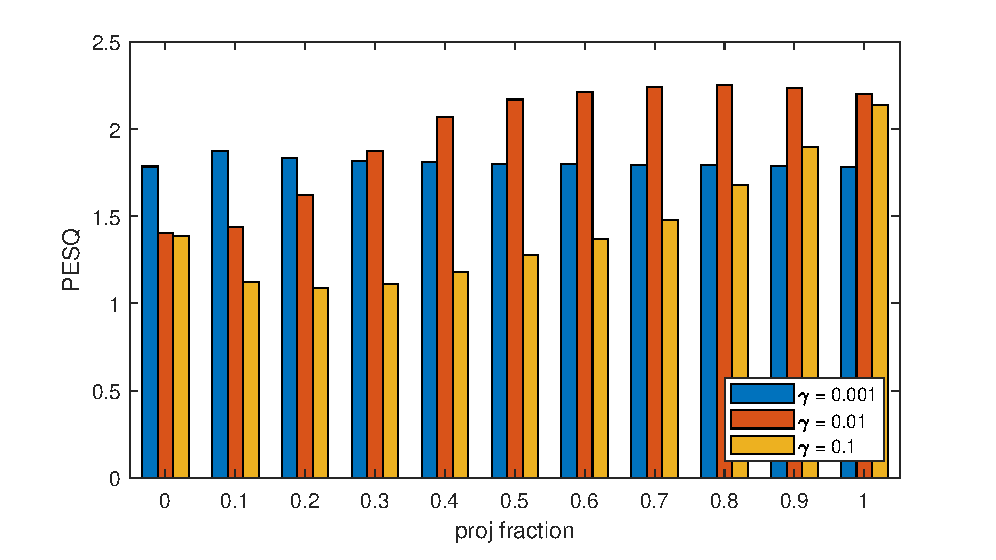
\includegraphics[width=1\linewidth]{figures/gamma_test}
	\caption{PESQ metric results made to choose the best value of $\gamma$ in DRA for testing with multiple audio files (these values are shown in the legend). %\todo{Dopsal bych to přímo do obrázku, pokud to půjde, že $\gamma=\dots$.}
	The results in terms of STOI and SNR were principally the same.
	The label \textit{proj fraction} refers to parameter $\beta$ from Alg.\,\ref{alg:DRA}.}
	\label{fig:gammatest}
\end{figure}

The best results were obtained with $\gamma=0.01$, which reached the best restoration quality, especially with increasing ratio of projected signal.

\subsection{Test setup}
We have chosen randomly 10 audio files for final evaluation from the Valentini dataset \cite{ValentiniBotinhao2017} described before.
% used commonly in speech enhancement challenges (the dataset is split to two subsets: clean and noisy).
%%\todo{Jde najít nebo spočítat, jaká je zhruba úroveň šumu u našich vzorků? Spočítat by to jít mohlo, prostě SNR pro clean versus noisy-clean\dots}
%The average SNR of our files is approximately $11$ dB.
%For each signal, we used the clean sample as a reference and its noisy variant as the input to the algorithm. % (clean with addition of noise, which is required to supress).
%As a simulation of inpainting task, we used random drop-out of % uniformly distributed mask of zero and ones, where partition of 0 is
%$40\%$ of samples as used in \cite{Mokry2021}.
%This means that the reliable set $I_\textup{R}$ consisted of $60\%$ of all the sample indices.
%% Then this mask is applied as dot product with noise signal.
As described before in \ref{subsec:soft_thresh}, we have chosen $\gamma = 0.01$.
The simulation was split to three variants: two conventional ones and one including the learned denoiser.
The conventional ones were two versions of DRA \ref{alg:DRA} with same parameters except for the number of iterations ($50$ or $500$) and the choice of $\lambda_n$ (decreasing or constant).
The DRA with denoiser proposed in Alg.\,\ref{alg:pnp} was tested with $50$ iterations,
as in the shorter conventional method.
In all the algorithms, the initial $\lambda_0$ was set to $1$. %\todo{Zkontrolovat, kdybychom měnili.}
For the case of DRA \ref{alg:DRA} with 500 iterations, we kept constant $\lambda_n = 0.1$.
In the case of the plug-and-play version \ref{alg:pnp}, and the reference DRA \ref{alg:DRA} with 50 iterations, the parameter was set to decrease in every iteration as $\lambda_{n+1} = 0.9\cdot\lambda_n$.
%\todo{Máme nějaké historické obrázky (nebo můžeme znova pustit nějaký starý test), který by ilustroval, proč potřebujeme tu lambdu snižovat? Nebo to tu jen řekneme, že se jinak kvalita zhoršovala s postupujícími iteracemi? V tomto místě by to totiž chtělo vysvětlit, proč to tak bylo nastaveno.}
The motivation for decreasing $\lambda$ is clear from Fig.\,\ref{fig:lamdadesc}.
Test was made using DRA and every option should converge to same optimal point in time.
%\todo{To je pro klasický DRA nebo pro denoise? To by zde mělo být zdůrazněno, mimo jiné proto, že pokud je to klasický DRA, pak by měl časem konvergovat bez ohledu na volbu $\lambda$ ke stejnému optimu (ale v praxi při konečném počtu iterací to může hrát roli).}
If we fix $\lambda$, SNR decreased and converge to wrong point.
If $\lambda$ decreases, we minimize the impact of soft threshold operator in latter iterations which appears to be effective in practice.

\begin{figure}[!h]
	\centering
	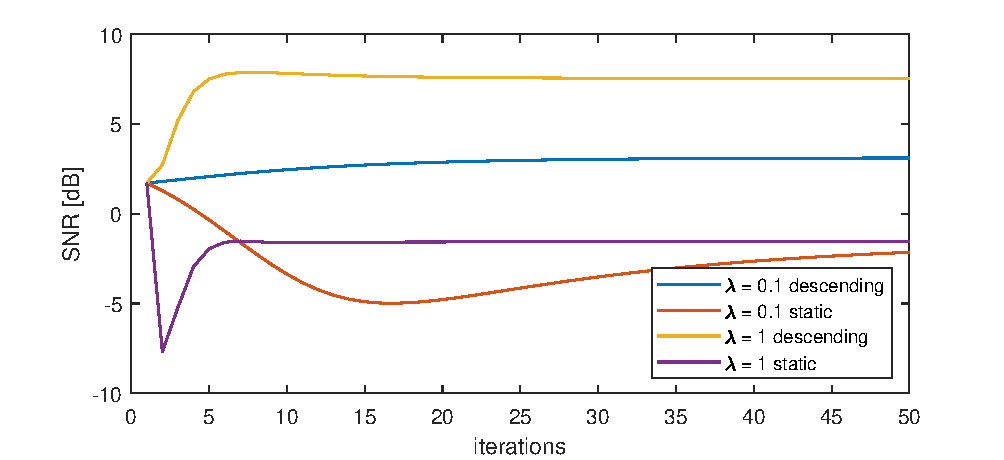
\includegraphics[width=1\linewidth]{figures/lamda_desc}
	\caption{SNR from DRA tested for 50 iterations with static and decreasing choice of $\lambda \in \{0.1,1 \}$.
	Tested signals are same as in experiment with $\gamma$.}
%	\todo{Predsa len rozmýšlam pustiť ten algoritmus odznova s $\gamma=1$}\\
%	\todo{OM: ano, zkusil bych to}\\
%	\todo{OM: jako značení bych možná používal to $\lambda_0$, pomocí toho se mi povedlo formalizovat to klesání totiž}}
	\label{fig:lamdadesc}
\end{figure}

%In every algorithm is $\lambda$ scaled with coefficent $\alpha$
%\todo{(MŠ: zvolil som alfu, ale v algoritme nie je vôbec. Je potrebné ju do algoritmov pridať?)}
%\todo{OM: $\alpha$ se mi hodilo výše v rovnici \eqref{eq:analysis.dist}, zde jsem to zkusil přepsat bez potřeby nějak to označit}
%each iteration.
%We set $\alpha$ to $0.9$ in algorithms with $50$ iterations and $1$ for DRA $500$ iterations, because the effect of $\lambda$ after $500$ divisions will be negligible.



\subsection{Comparison results}

\begin{figure*}[t]
	\begin{subfigure}{.33\textwidth}
		\centering
		% include first image
		\includegraphics[width=1.1\linewidth]{figures/lam1_stoi}  
	\end{subfigure}
	\begin{subfigure}{.33\textwidth}
		\centering
		% include second image
		\includegraphics[width=1.1\linewidth]{figures/lam1_PESQ}  
	\end{subfigure}
	\begin{subfigure}{.33\textwidth}
		\centering
		% include second image
		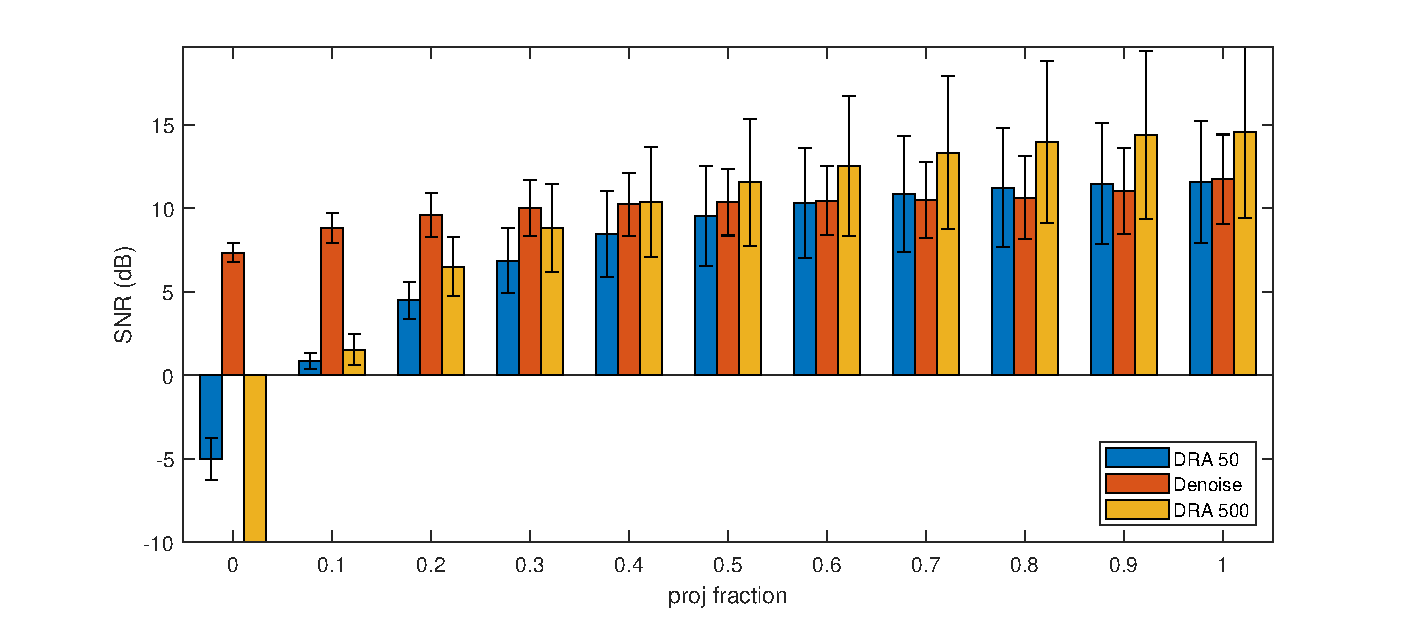
\includegraphics[width=1.1\linewidth]{figures/lam1_SNR}  
	\end{subfigure}
	\caption{Average results from 10 tested signals. Metrics are from left: STOI, PESQ, SNR.
		\todo{$\lambda_0 = 1 $ pre DRA 50 a PnP 50, pre DRA 500 $\lambda_0=0.1$ nevedelo mi to spocitat PESQ pre vyššie $\lambda_0$ keď bolo static}
		}
	\label{fig:final3witherrors}
\end{figure*}


%\todo{OM: Zde použít víc metrik, přinejmenším STOI, PESQ a SNR (možná vynechat SNR max a SNR gap). Dát 3 grafy vedle sebe pomocí figure*.}
%\todo{MŠ: Graf sa ešte doplní lepší, musím vymyslieť ešte ako.}

%\todo{OM: Možná místo Denoise bych používal Plug-and-play.}

%\todo{OM: Na co bych se tak zaměřil v diskuzi výsledků: Plug-and-play je méně citlivý na volbu poměru v projekci a v případě srovnání s DRA \ref{alg:DRA} se stejnými parametry (50 iterací, klesající $\lambda_n$) může dosáhnout epších výsledků.Ve srovnání s DRA s 500 iteracemi máme nižší variabilitu, ovšem globálně, při možnosti optimalizovat paramtry jako je právě míchací poměr $\beta$, jsou naše výsledky horší.}

Graphs with STOI, PESQ and SNR are presented in Fig.\,\ref{fig:final3witherrors}.
We see that plug-and-play is less sensitive to the fraction of projection compared to DRA,
and in comparison with DRA (50 iterations, decreasing $\lambda_n$), it reaches better result.
DRA with 500 iterations has higher variance of the results, but globally, it outperformed the plug-and-play method with optimal choice of the parameters such as the fraction ratio $\beta$.



%\begin{figure*}[b!]
%	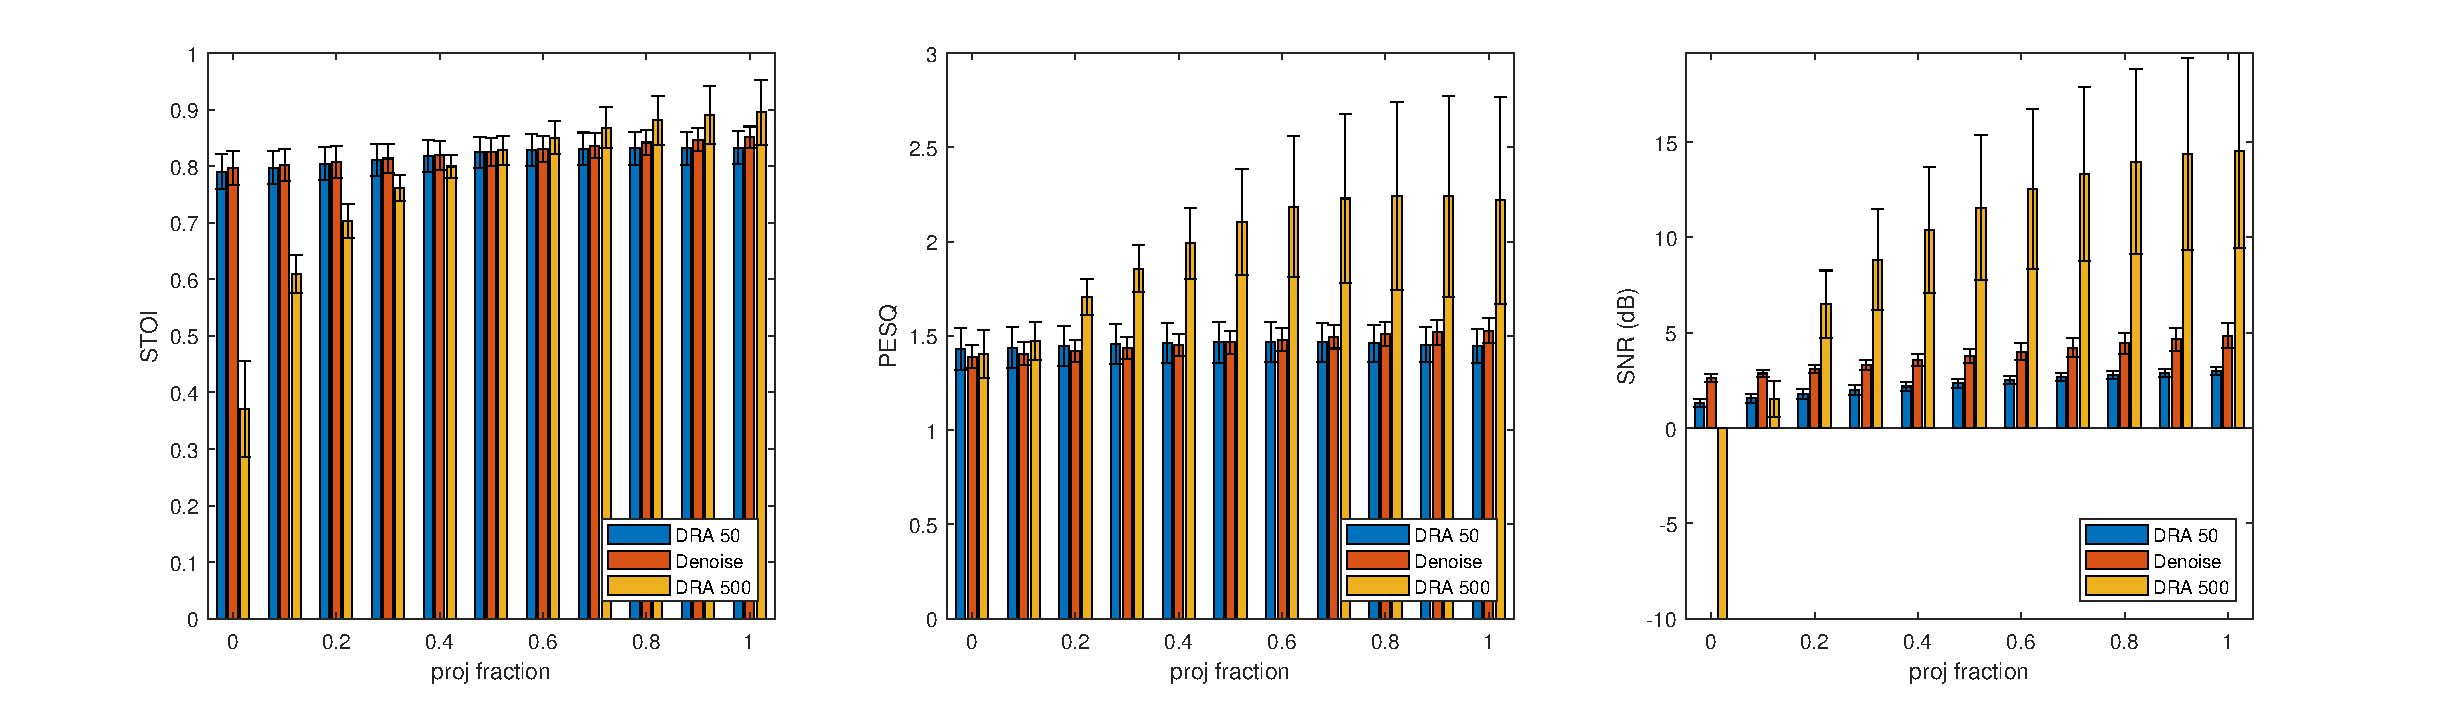
\includegraphics[width=1\linewidth]{figures/final2_with_errors}
%	\caption{Široký obrázek.}
%	\label{fig:final2witherrors}
%\end{figure*}





\section{Conclusion}
\label{sec:conclusion}

Our reformulation of plug-and-play method for audio inpainting has shown succesful with properly chosen ratio of projection and $\lambda$.
Next steps will be extend the test for other similar tasks (declipping, dequantization), following the pattern of root method \cite{Chan2016}, solving multiple tasks with one setup of the algorithm.
It is suggested not to use off-the-shelf denoiser, but hand-crafted, which is learned on data related to our problem (e.g. specific noise due to dropout of a certain percentage of samples).
In addition,
we might be able to make the self-learned denoiser non-expansive, thus satisfying the theoretical convergence guarantees \cite{Venkatakrishnan2013,Chan2016}.
Another improvement might be transfer learning,
i.e. use success denoiser and continue learning from checkpoint with our dataset,
with idea to reduce artefacts generated in inpainting task.

%\todo{Záver a Abstrakt TODO ráno}
%\todo{Naše metoda je super (až na to, že nefunguje, ale to nebudeme říkat).}
%\todo{Dalším postupem bude testovat použití na jiné související úlohy dle principu plug-and-play (declipping, dekvantizace). Nabízí se zkusit nepoužívat off-the-shelf denoiser, ale vlastní, který je učený na datech příbuzných s naší úlohou (např.\ specifický šum vzniklý výpadkem jistého procenta vzorků). Současně u vlastního učení bychom mohli umět zařídit, že denoiser bude non-expansive a tudíž splníme teoretické záruky konvergence \cite{Venkatakrishnan2013,Chan2016}. Taktéž by se nabízel transfer learning, tj.\ vzít dobrý denoiser a jenom ho doučit, aby byl schopný redukovat artefakty vzniklé v inpaintovací úloze.}

%\section*{Appendix: Derivation of the projection-like update}
%
%\noindent
%\todo{\textbf{(do článku bych asi nedával, spíš pro info})}
%\todo{%
%	Dle \cite[Tab.\,1]{Combettes2011}
%	\begin{equation}
%		\operatorname{prox}_f(\mathbf{y}) = (\mathbf{I} + \alpha \mathbf{M}_{\textup{R}}^\top\mathbf{M}_{\textup{R}})^{-1}(\mathbf{y} + \alpha\mathbf{M}_{\textup{R}}^\top\mathbf{M}_{\textup{R}}\mathbf{s}).
%	\end{equation}
%	Protože $\mathbf{M}_{\textup{R}}^\top\mathbf{M}_{\textup{R}}$ je diagonální matice, která má 1 na pozicích $I_\textup{R}$ a 0 na pozicích $I_\textup{M}$ diagonály, můžeme rozepsat po vzorcích (pozor, $n$ zde indexuje vzorky, ne iterace)
%	\begin{equation}
%		\left[\operatorname{prox}_f(\mathbf{y})\right]_n = \begin{cases}
%			\frac{1}{1+\alpha}(y_n + \alpha s_n) \quad &\text{pro } n\in I_\textup{R}, \\
%			y_n\quad &\text{pro } n\in I_\textup{M}. 
%		\end{cases}
%	\end{equation}
%	V našem případě $(1-\beta)\mathbf{x} + \beta \operatorname{proj}_{\Gamma}(\mathbf{x})$ jsou pozice $I_\textup{M}$ zřejmé, protože projekce tyto vzorky nemění, tzn.\ máme
%	\begin{equation}
%		(1-\beta) x_n + \beta x_n = x_n \text{ pro } n\in I_\textup{M}.
%	\end{equation}
%	Pro vzorky v $I_\textup{R}$ naopak projekce vrací hodnotu $s_n$, tudíž
%	\begin{equation}
%		(1-\beta) x_n + \beta s_n = \frac{1}{1+\alpha}(x_n + \alpha s_n)\text{ pro } n\in I_\textup{R}.
%	\end{equation}
%	Odsud
%	\begin{equation}
%		\beta = \frac{\alpha}{1+\alpha} = 1 - \frac{1}{1+\alpha} \Longrightarrow \alpha = \frac{\beta}{1-\beta}.
%	\end{equation}
%}

%\section*{Acknowledgment}
%
%The preferred spelling of the word ``acknowledgment'' in America is without 
%an ``e'' after the ``g''. Avoid the stilted expression ``one of us (R. B. 
%G.) thanks $\ldots$''. Instead, try ``R. B. G. thanks$\ldots$''. Put sponsor 
%acknowledgments in the unnumbered footnote on the first page.

\bibliographystyle{IEEEtr}
\bibliography{bib_eeict2023}



\end{document}
